\documentclass{article}
\usepackage{graphicx}
\usepackage[margin=1.5cm]{geometry}
\usepackage{amsmath}
\usepackage{url}

\begin{document}

\title{PhET Activity: Unit 1, Acceleration and Kinematics}
\author{Prof. Jordan C. Hanson}

\maketitle

\section{Position, Velocity, and Acceleration}

\begin{enumerate}
\item Open the OpenStax text for the course, and navigate to Ch. 2.4: \url{https://openstax.org/details/books/college-physics}.
\item Scroll all the way to the bottom and find the PhET simulation.  Click on the link for the Moving Man Simulation, entitled \textbf{Click to View Content.}
\item The introduction tab at the top left will help you learn the controls.  Using the mouse, you can drag the man left and right in one dimension.  His position, velocity, and acceleration will be indicated by the blue, red, and green markers, respectively.
\item Now click on the tab at the top left entitled \textbf{Charts.}
\item Slowly drag the man to the right \textit{at a steady pace.}  Do you observe the following?
\begin{itemize}
\item A linearly increasing position?
\item A (roughly) constant velocity?
\item An acceleration that is basically zero?
\end{itemize}
\item Hit reset at the bottom right, and redo the experiment.  This time, move the man all the way to the right, then move him all the way to the left.  As accurately as you can, with labeled axes and units, draw his position below: \\ \vspace{2.0cm}
\item From the position versus time graph you've created, identify the region of positive velocity by looking at the slope.  Calculate the average velocity from the slope of your graph.  Repeat this exercise for the region of negative velocity.  When does acceleration deviate from zero?
\end{enumerate}

\begin{figure}[hb]
\centering
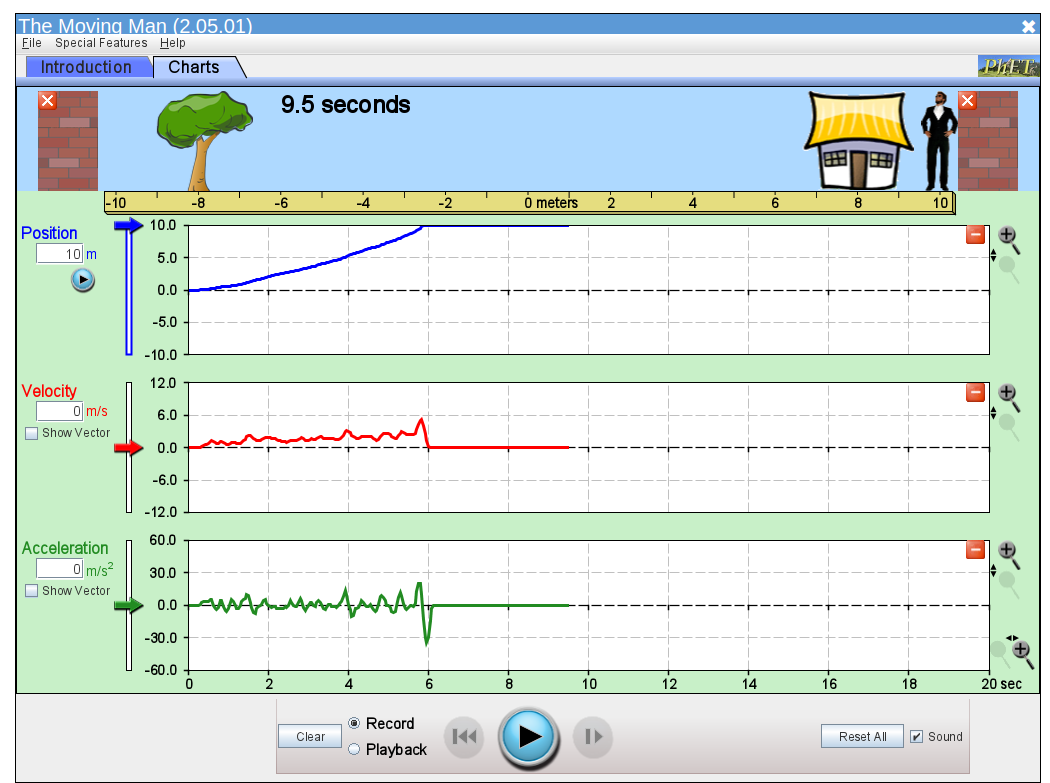
\includegraphics[width=0.4\textwidth]{figures/man.png}
\caption{Example of the PhET simulation.}
\end{figure}

\end{document}
